%-------------------------------------------------------------------------------
% seq66 setmaster
%-------------------------------------------------------------------------------
%
% \file        seq66 setmaster.tex
% \library     Documents
% \author      Chris Ahlstrom
% \date        2020-01-13
% \update      2023-11-25
% \version     $Revision$
% \license     $XPC_GPL_LICENSE$
%
%     Provides a discussion of the MIDI GUI setmaster that Seq66
%     supports.
%
%-------------------------------------------------------------------------------

\section{Seq66 Set Master}
\label{sec:setmaster}

   The \textbf{Set Master} is a way to get a global view of all the screensets
   in a \textsl{Seq66} MIDI file, and to be able to do some simple operations
   (movement, naming, etc.) with the sets.
   In the latest version of \textsl{Seq66}, there are always 32 sets.
   This simplifies the handling of sets.
   Some sets may be empty.

\begin{figure}[H]
   \centering 
   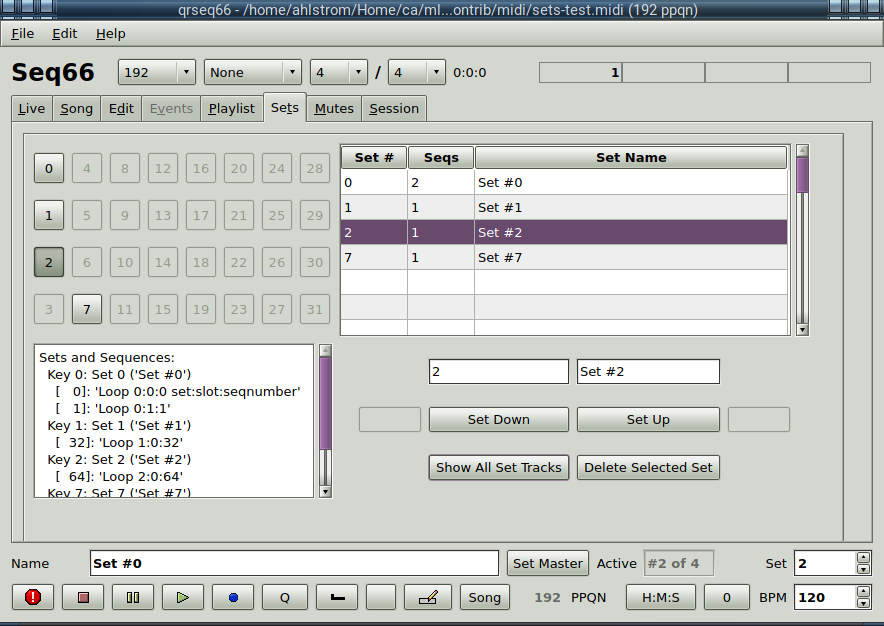
\includegraphics[scale=0.50]{tabs/sets/setmaster-tab.png}
   \caption{Sets Tab}
   \label{fig:setmaster_tab}
\end{figure}

   The operations that can be done consist of viewing the sets, making a
   screenset active, rearranging the sets, clearing sets, and getting a survey
   of the contents of the sets.

   \setcounter{ItemCounter}{0}      % Reset the ItemCounter for this list.

   \itempar{Sets Grid}{set master!grid}
   The set grid is always 4 x 8.  Like the mute-groups, there's not
   a lot of benefit supporting more sets.  The reader may wish to email us
   arguing for a different point of view.
   \index{play screen}
   This grid shows the non-empty sets that are present in the MIDI file,
   represented by enabled buttons.
   With \textbf{Triggers} mode set, this  allows one to choose which set
   is currently
   active (i.e. which is the "play screen").
   Click on it and it is active.
   Also remember that keystrokes (\texttt{[} and \texttt{]} by default)
   in the main window can move the playscreen to the previous or next set.
 
   \itempar{Set List}{set master!list}
   The table at the right shows the set numbers, how many patterns/sequences
   are in each set, and the set name.  The set name is editable once it is
   double-clicked.

   \itempar{Set Number/Name Fields}{set master!number/name}
   Currently just shows the number and name of the selected set.
   Eventually, these fields will be editable.

   \itempar{Up/Down Buttons}{set master!up/down buttons}
   These buttons allow the user to move the selected set up and down
   in the list.

   \itempar{Show Set Info}{set master!show set info}
   Clicking this button lists all the sets and their tracks in the
   read-only edit box at the left.

   \itempar{Clear Set}{set master!clear set}
   Clicking this button deletes the patterns from the 
   set selected in the table.
   Note that the 0th set cannot be cleared.
   Would one ever want to do that?
   In \textsl{Seq66}, there must always be a set 0.

   \itempar{Triggers}{set master!set triggers}
   This checkable button toggles the action done by clicking a button
   in the set grid.
   If checked, then clicking an active set button will make that
   set active during playback.
   That effect depends on whether the sets are configured to auto-arm when
   selected, or not.
   If not checked, then clicking an active set button merely summarizes the
   patterns in the set, in the text field below the set grid.

   \itempar{Set 0}{set master!set 0}
   If trigger mode is in effect, clicking this button makes
   set 0 active.
   An alternative to clicking on grid button 0.

\subsection{Set Handling}
\label{subsec:setmaster_handling}

   This section talks about how sets work.  The topics are

   \begin{itemize}
      \item \textbf{Set Management}
      \item \textbf{Empty-Set Handling}
   \end{itemize}

\subsubsection{Set Management}
\label{subsubsec:setmaster_management}

   This section will discuss the work-flows of using sets to organize a song
   and to control playback.  MORE TO COME.

\subsubsection{Empty Set Handling}
\label{subsubsec:setmaster_empty_sets}

   When \textsl{Seq66} loads a song, it loads the existing sets in the song and
   sets their names as stored in the \texttt{c\_notes} \textsl{SeqSpec}
   (see \sectionref{subsec:midi_format_meta_format}).
   In addition, one dummy and invisible set is created for internal management
   purposes.

   When a new song is created, one usable set, Set \#0, is always created, as a
   starting point.  One generally starts with this set and adds patterns to it.

   When one selects the next set (e.g. using the \textbf{Live} frame's
   \textbf{Set} spin control), that set does not exist, but is immediately
   created.  So now the song has two sets, with the second one being empty.
   If the song is now saved, so is the empty set's file name.  However, empty
   sets are not saved; a set must be populated with at least one pattern to be
   saved.

   The following figure shows what happens when a song with 4 sets (0, 1, 2,
   and 7) is loaded, and then the user increments the spin-button all the way
   to set 8.

\begin{figure}[H]
   \centering 
   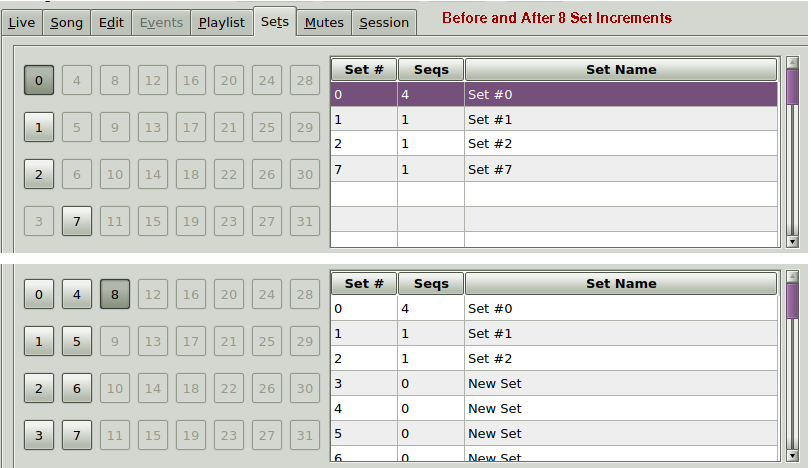
\includegraphics[scale=0.85]{tabs/sets/setmaster-with-additional-sets.png}
   \caption{New Sets Creation}
   \label{fig:setmaster_set_creation}
\end{figure}

   There are new sets 3, 4, 5, 6, and 8.  However, if one saves and then
   reloads this song, the empty sets are gone.  Just something to be aware of.

%-------------------------------------------------------------------------------
% vim: ts=3 sw=3 et ft=tex
%-------------------------------------------------------------------------------
